		\tikzset{every picture/.style={line width=0.75pt}} %set default line width to 0.75pt        
		
		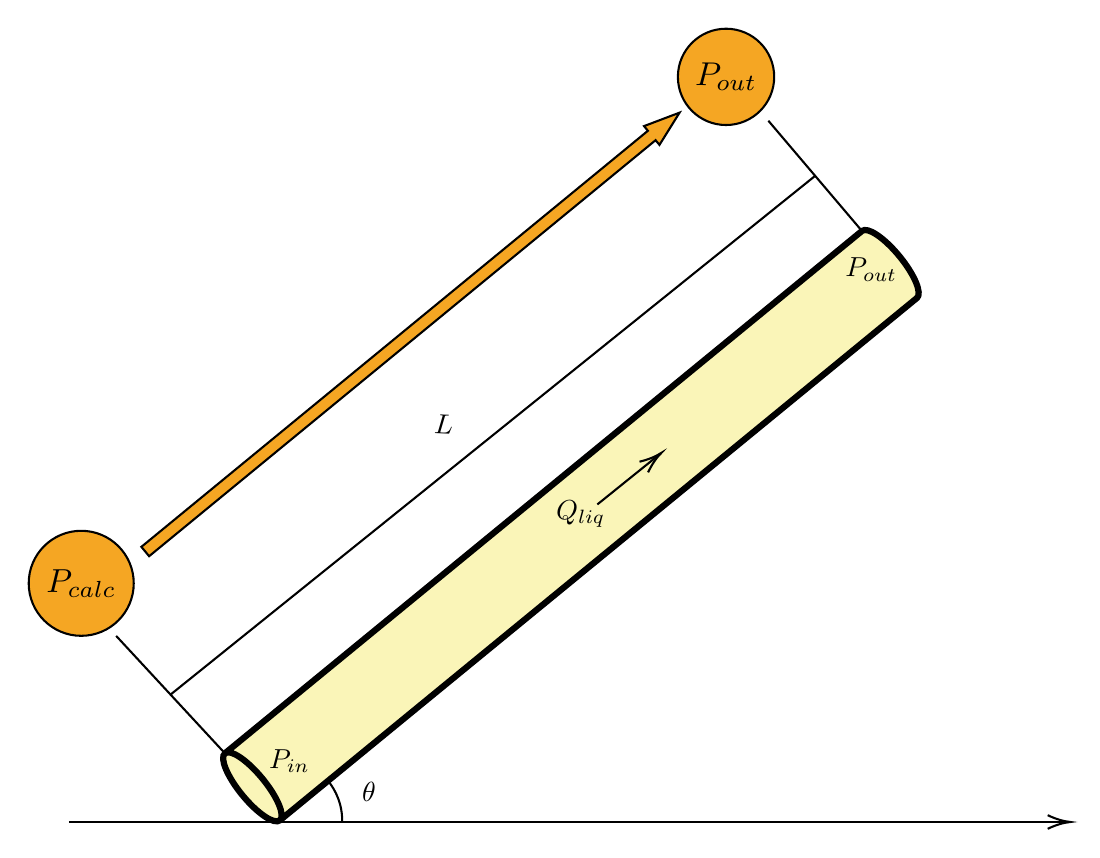
\begin{tikzpicture}[x=0.75pt,y=0.75pt,yscale=-1,xscale=1]
		%uncomment if require: \path (0,390); %set diagram left start at 0, and has height of 390
		
		%Shape: Can [id:dp7382807235009181] 
		\draw  [fill={rgb, 255:red, 250; green, 245; blue, 184 }  ,fill opacity=1 ][line width=2.25]  (176.23,350.28) -- (483.15,98.62) .. controls (485.82,96.43) and (493.92,101.88) .. (501.23,110.8) .. controls (508.54,119.72) and (512.3,128.72) .. (509.63,130.92) -- (202.71,382.57)(176.23,350.28) .. controls (178.9,348.08) and (187,353.54) .. (194.31,362.45) .. controls (201.63,371.37) and (205.39,380.38) .. (202.71,382.57) .. controls (200.03,384.77) and (191.94,379.32) .. (184.62,370.4) .. controls (177.31,361.48) and (173.55,352.47) .. (176.23,350.28) -- cycle ;
		%Shape: Arc [id:dp26711502457409386] 
		\draw  [draw opacity=0] (225.54,363.1) .. controls (227.72,365.66) and (229.51,368.62) .. (230.76,371.95) .. controls (232.22,375.8) and (232.84,379.77) .. (232.7,383.64) -- (202.71,382.57) -- cycle ; \draw   (225.54,363.1) .. controls (227.72,365.66) and (229.51,368.62) .. (230.76,371.95) .. controls (232.22,375.8) and (232.84,379.77) .. (232.7,383.64) ;
		%Straight Lines [id:da2708011557353165] 
		\draw    (123.83,293.7) -- (176.23,350.28) ;
		
		
		%Straight Lines [id:da09547020181005683] 
		\draw    (438.06,45.51) -- (483.15,98.62) ;
		
		
		%Straight Lines [id:da29893852101776] 
		\draw    (150.03,321.99) -- (460.6,72.07) ;
		
		
		%Straight Lines [id:da6573662742713218] 
		\draw    (355.67,230.37) -- (385,206.74) ;
		\draw [shift={(386.56,205.48)}, rotate = 501.14] [color={rgb, 255:red, 0; green, 0; blue, 0 }  ][line width=0.75]    (10.93,-3.29) .. controls (6.95,-1.4) and (3.31,-0.3) .. (0,0) .. controls (3.31,0.3) and (6.95,1.4) .. (10.93,3.29)   ;
		
		%Straight Lines [id:da5485107193914818] 
		\draw    (101,383.37) -- (581.56,383.37) ;
		\draw [shift={(583.56,383.37)}, rotate = 180] [color={rgb, 255:red, 0; green, 0; blue, 0 }  ][line width=0.75]    (10.93,-3.29) .. controls (6.95,-1.4) and (3.31,-0.3) .. (0,0) .. controls (3.31,0.3) and (6.95,1.4) .. (10.93,3.29)   ;
		
		%Right Arrow [id:dp6841435853741948] 
		\draw  [fill={rgb, 255:red, 245; green, 166; blue, 35 }  ,fill opacity=1 ] (135.99,250.8) -- (380.02,50.35) -- (378.16,48.09) -- (395.29,41.6) -- (385.59,57.14) -- (383.73,54.88) -- (139.71,255.32) -- cycle ;
		
		% Text Node
		\draw (245.67,368.7) node   {$\theta $};
		% Text Node
		\draw (281.67,192.04) node [rotate=-2.44]  {$L$};
		% Text Node
		\draw (207.33,354.04) node [rotate=-0.74]  {$P_{in}$};
		% Text Node
		\draw (487.67,117.37) node [rotate=-0.74]  {$P_{out}$};
		% Text Node
		\draw (347.67,235.04) node [rotate=-0.61]  {$Q_{liq}$};
		% Text Node
		\draw  [color={rgb, 255:red, 0; green, 0; blue, 0 }  ,draw opacity=1 ][fill={rgb, 255:red, 245; green, 166; blue, 35 }  ,fill opacity=1 ]  (107, 268.37) circle [x radius= 25.3, y radius= 25.3]   ;
		\draw (107,268.37) node [scale=1.2,rotate=-359.71]  {$P_{calc}$};
		% Text Node
		\draw  [fill={rgb, 255:red, 245; green, 166; blue, 35 }  ,fill opacity=1 ]  (417.67, 24.37) circle [x radius= 23.2, y radius= 23.2]   ;
		\draw (417.67,24.37) node [scale=1.2,rotate=-0.74]  {$P_{out}$};
		
		
		\end{tikzpicture}